\chapter*{Earlier Volumes in the Series}\label{evc}

\vspace{-1cm}

\section*{Volume-1 Western Indology and Its Quest for Power}

\begin{figure}[!htbp]
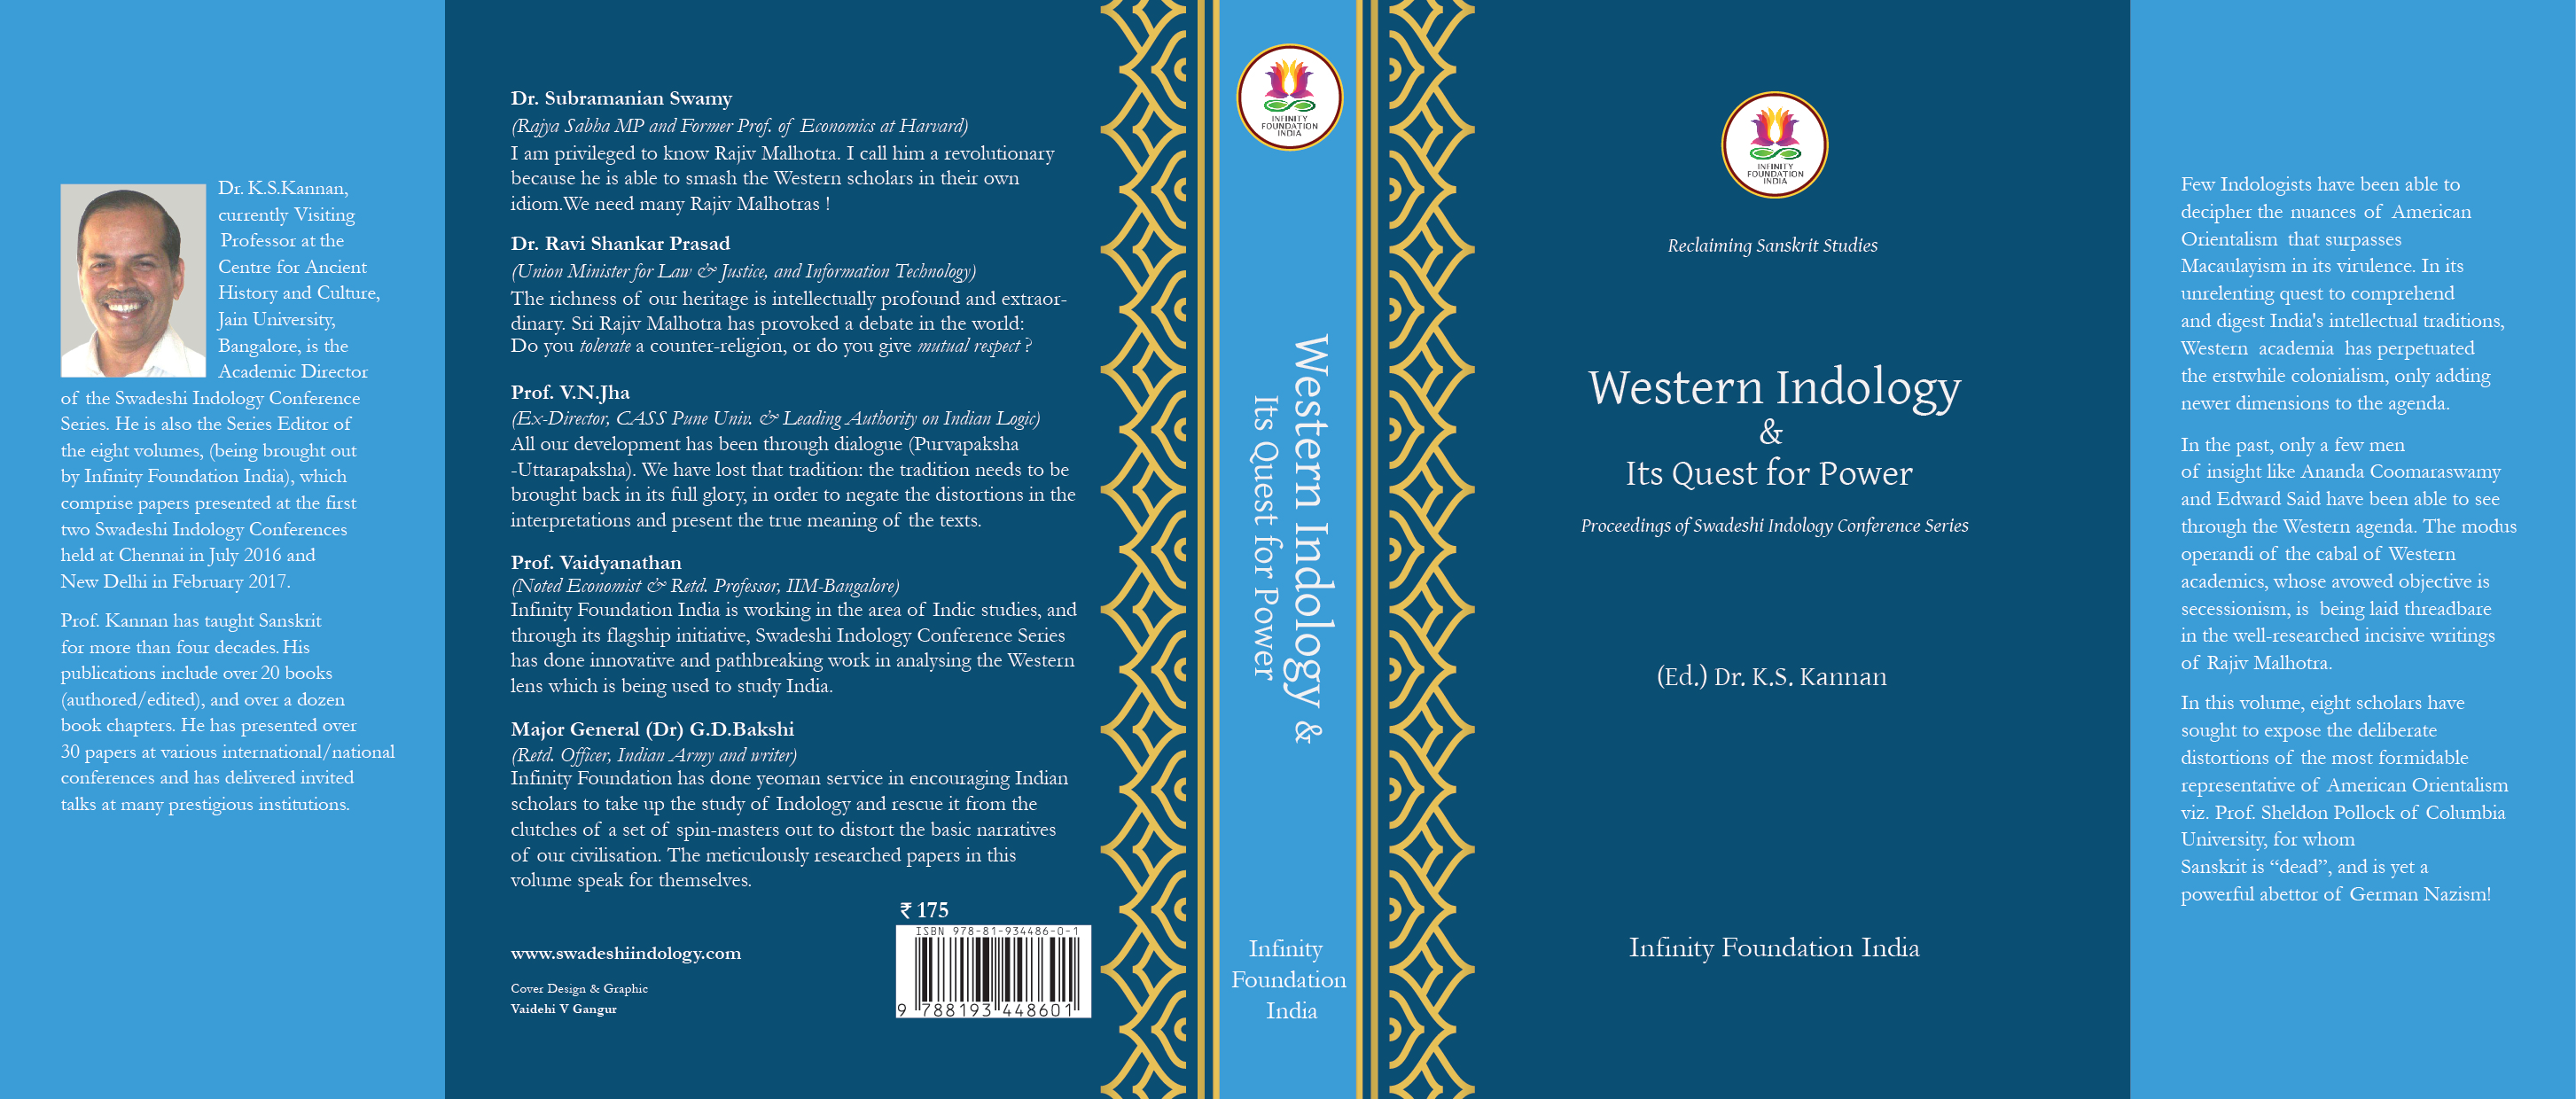
\includegraphics[scale=.727]{images/fig01.png}
\end{figure}

Few Indologists have been able to decipher the nuances of American Orientalism that surpasses Macaulayism in its virulence. In its unrelenting quest to comprehend and digest India’s intellectual traditions, Western academia has perpetuated the erstwhile colonialism, only\break adding newer nefarious dimensions to the agenda. 

In the past, only a few men of insight like Ananda Coomaraswamy and Edward Said have been able to see through the Western agenda. The modus operandi of the cabal of Western academics, whose avowed objective is secessionism, is being laid threadbare in the well-researched incisive writings of Rajiv Malhotra.

In this volume, eight scholars have sought to expose the deliberate distortions of the most formidable representative of American Orientalism viz. Prof. Sheldon Pollock of Columbia University, for whom Sanskrit is “dead”, and is yet a powerful abettor of German Nazism!


\section*{Volume-2 \textit{Śāstra}-s Through the Lens of Western Indology – A Response}

\begin{figure}[!htbp]
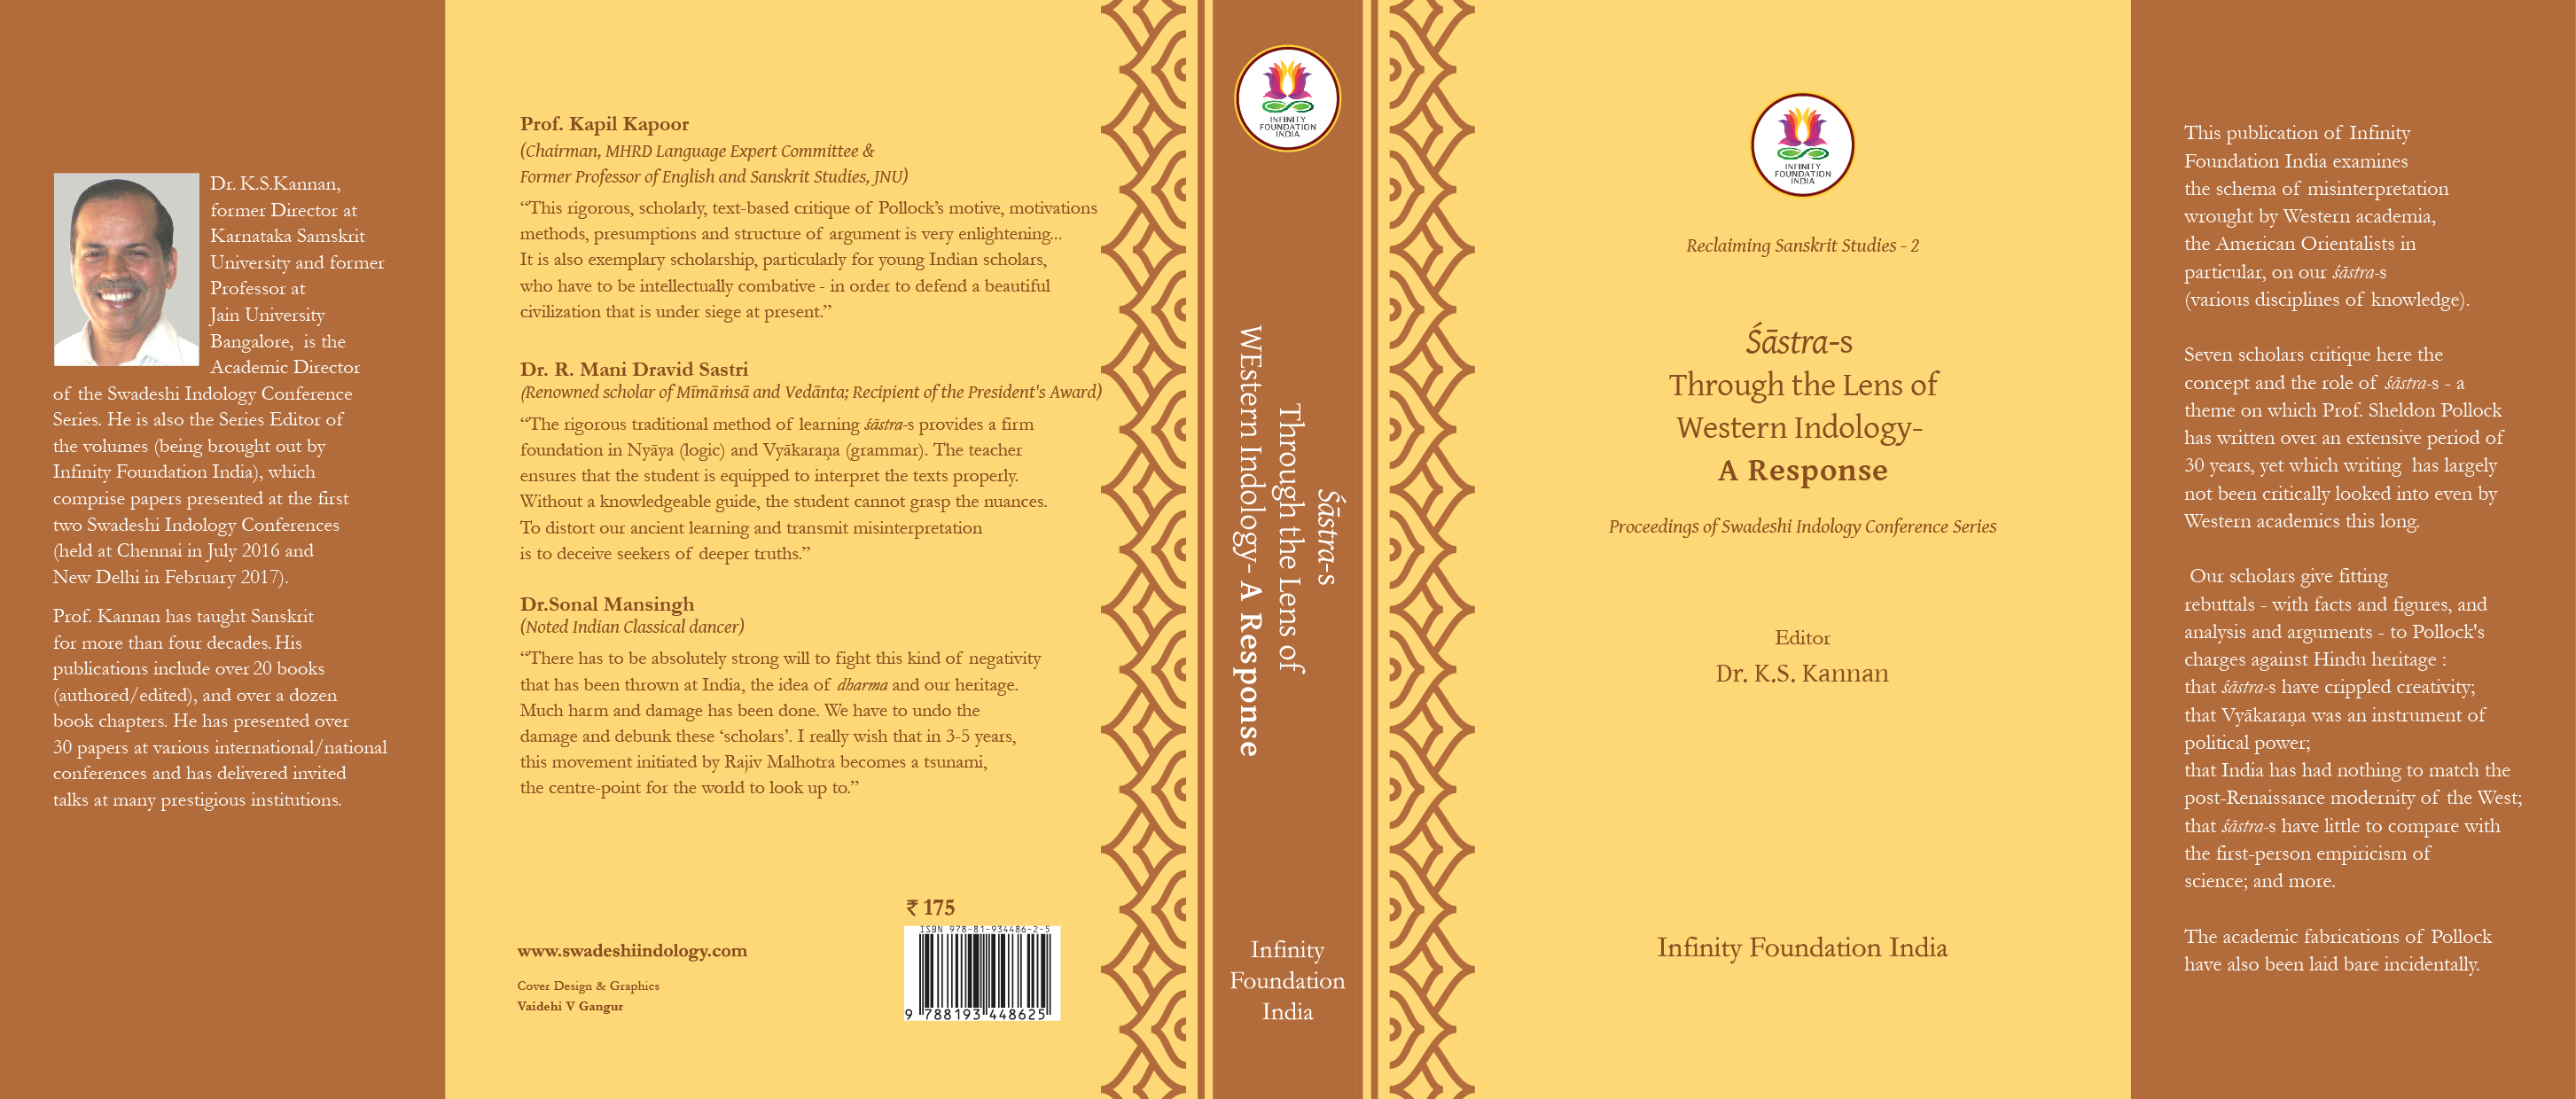
\includegraphics[scale=.727]{images/fig02.png}
\end{figure}

This publication of Infinity Foundation India examines the schema of misinterpretation wrought by Western academia, the American Orientalists in particular, on our \textit{śāstra}-s (various disciplines of knowledge).

Seven scholars critique here the concept and the role of \textit{śāstra}-s - a theme on which Prof. Sheldon Pollock has written over an extensive period of 30 years, yet which writing has largely not been critically looked into even by Western academics this long.

Our scholars give fitting rebuttals - with facts and figures, and analysis and arguments - to Pollock's charges against Hindu heritage: that \textit{śāstra}-s have crippled creativity; that Vyākaraṇa was an instrument of political power; that India has had nothing to match the post-Renaissance modernity of the West; that \textit{śāstra}-s have little to compare with the first-person empiricism of science; and more.

The academic fabrications of Pollock have also been laid bare incidentally.

\newpage

\section*{Volume-3 Reclaiming \textit{Rāmāyaṇa}: Disentan\-gling the Discourses}

\begin{figure}[!htbp]
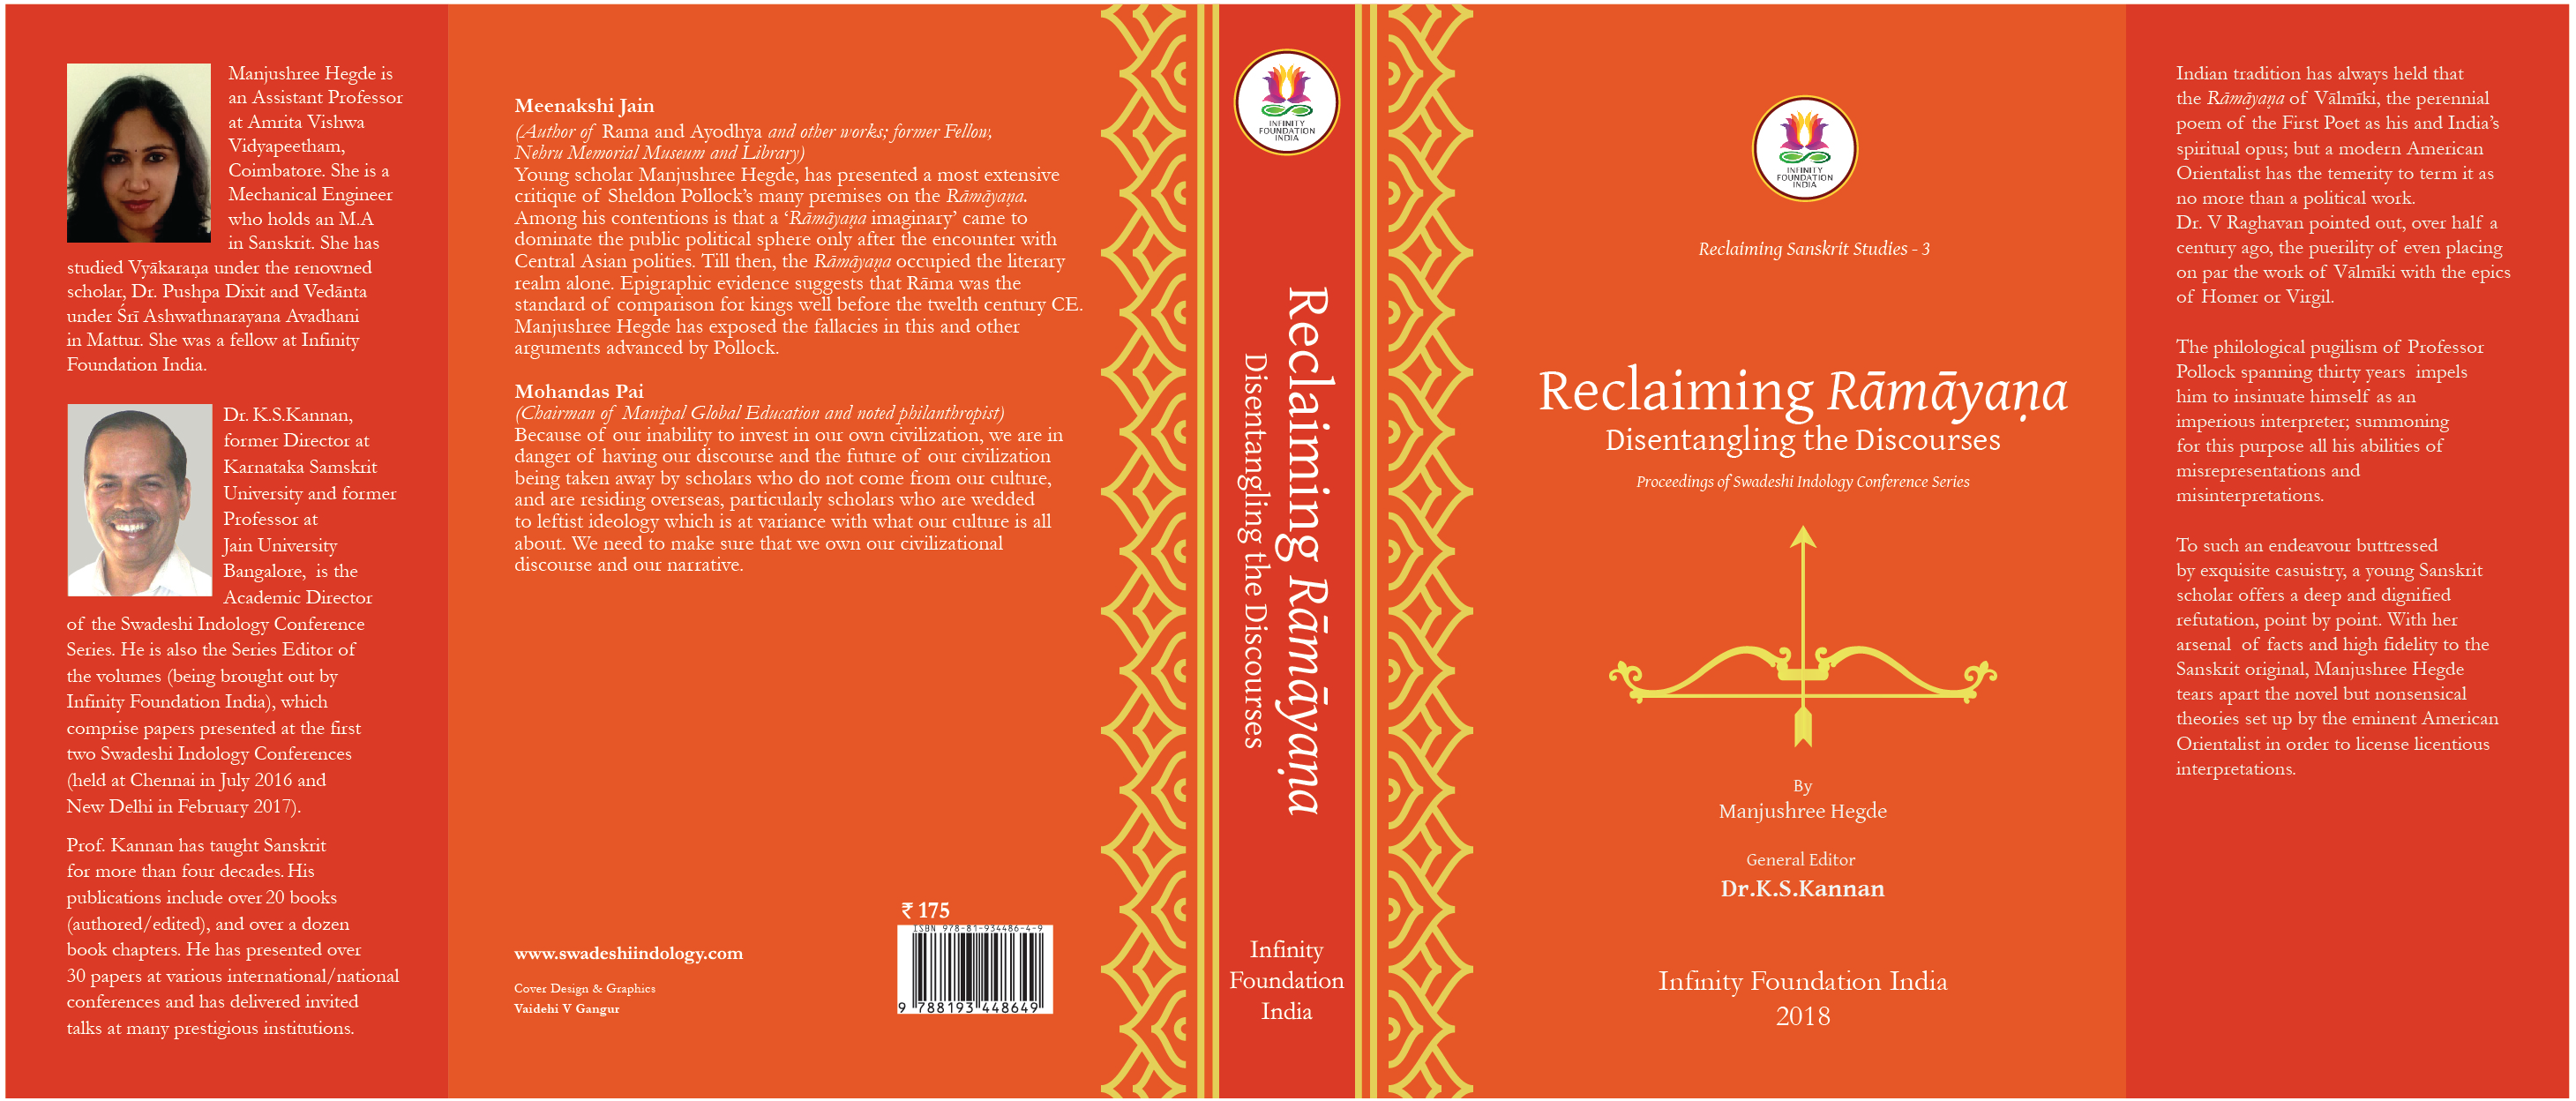
\includegraphics[scale=.81]{images/fig03.png}
\end{figure}

Indian tradition has always held that the \textit{Rāmāyaṇa} of Vālmīki, the perennial poem of the First Poet as his and India’s spiritual opus; but a modern American Orientalist has the temerity to term it as no more than a political work. Dr. V. Raghavan pointed out, over half a century ago, the puerility of even placing on par the work of Vālmīki with the epics of Homer or Virgil.

The philological pugilism of Professor Pollock spanning thirty years impels him to insinuate himself as an imperious interpreter; summoning for this purpose all his abilities of misrepresentations and misinterpretations.

To such an endeavour buttressed by exquisite casuistry, a young Sanskrit scholar offers a deep and dignified refutation, point by point. With her arsenal of facts and high fidelity to the Sanskrit original, Manjushree Hegde tears apart the novel but nonsensical theories — set up by the eminent American Neo-Orientalist in order to license licentious interpretations.

\newpage

\section*{Volume-4 Western Indology on \textit{Rasa: A Pūrvapakṣa}}

\begin{figure}[!htbp]
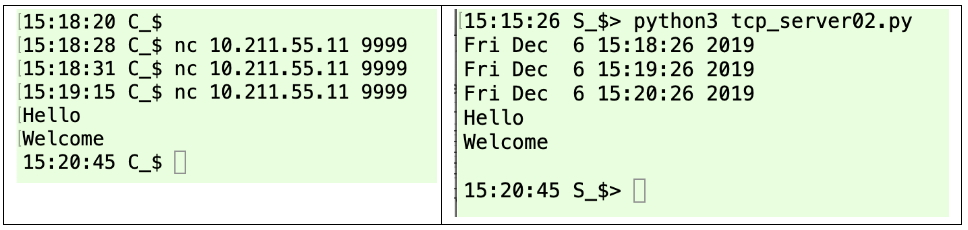
\includegraphics[scale=.51]{images/fig04.png}
\end{figure}

There is perhaps no realm of Indian heritage that Western Indology does not feel tempted to tamper with and tarnish.

Among others, the field of Alaṅkāra-śastra (poetics/rhetorics/\break dramaturgy) is also a natural efflorescence of the Indian ethos, and the Rasa Theory therein is one of the greatest contributions of India to the understanding – of literature, seen or heard, and of its impact on the audience – the lay or scholarly connoisseurs; and of psychology itself in general.

In his \textit{Rasa Reader}, Prof. Sheldon Pollock of Columbia University brings to bear a wealth of scholarship in order to subtly, and at places not so subtly, underrate and undermine Indian contribution to the comprehension of the role of human mind in the creation of, relish of, and response to, \textit{belles lettres}.

Over half a dozen scholars, all Indian, have looked deep in this volume into many aspects of the predominantly negative role of Pollock, and scripted their own understanding of the tradition and its nuances.

